
%---------------------------------------
\addcontentsline{toc}{chapter}{1 Thessalonians}

% Safely inserts your illustration full-bleed on its own page.
% This completely bypasses the page builder, headers, and geometry bugs!
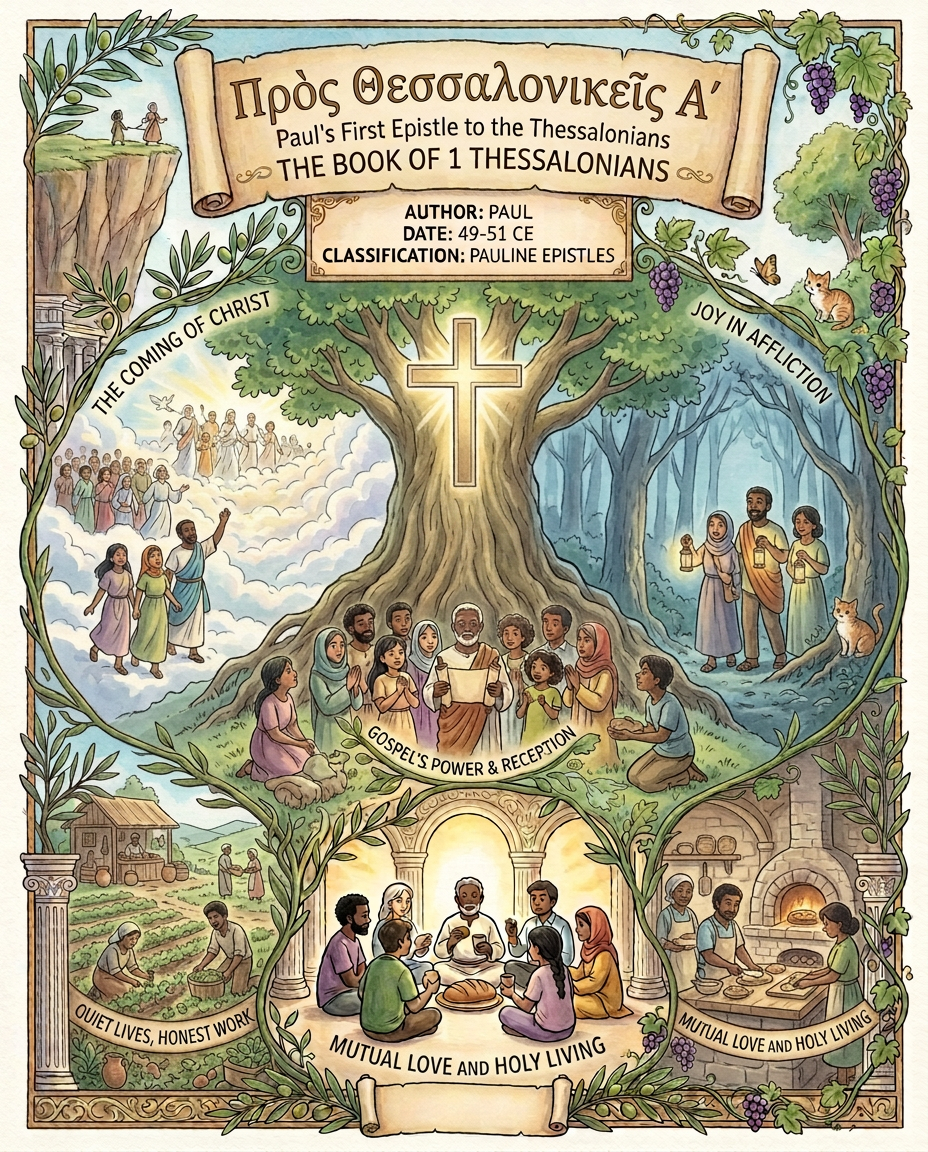
\includepdf[pages=1, fitpaper=false, width=\paperwidth, height=\paperheight, , keepaspectratio=false]{images/divider2/1thessalonians2.png}
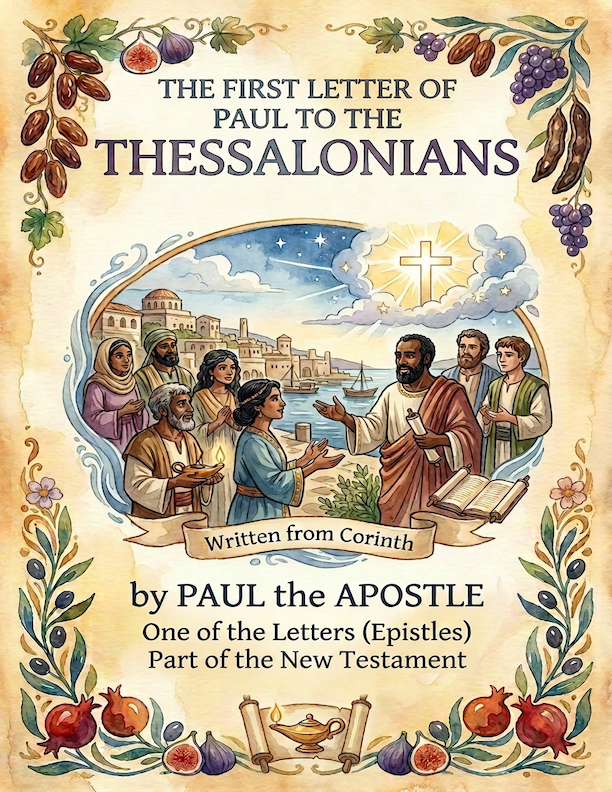
\includepdf[pages=1, fitpaper=false, width=\paperwidth, height=\paperheight, , keepaspectratio=false]{images/divider1/1thessalonians.png}

\includepdf[pages=1, fitpaper=false, width=\paperwidth, height=\paperheight, , keepaspectratio=false]{images/8.5x11-Dot-Grid.png}

\includepdf[pages=1, fitpaper=false, width=\paperwidth, height=\paperheight, , keepaspectratio=false]{images/8.5x11-Dot-Grid.png}

\mybook{1 Thessalonians}
\vspace{-1.36in}

\mychapter{} \myverse*{}Paul, Silvanus, and Timothy, to the assembly of the Thessalonians
in God the Father and the Lord Yeshua the Messiah:\footnote{1:1 “Messiah” means “Anointed One”.} Grace to you and peace from God our Father and the Lord
Yeshua the Messiah.

\myverse{}We always give thanks to God for all of you, mentioning you in
our prayers,
\myverse{}remembering without ceasing your work of faith and labor of love and perseverance
of hope in our Lord Yeshua the Messiah, before our God and Father.
\myverse{}We know, brothers\footnote{1:4 The word for “brothers” here and where context allows may also be correctly translated “brothers
	and sisters” or “siblings.”
} loved by God, that you are chosen,
\myverse{}and that our Good News came to you not in word only, but also in power, and
in the Holy Spirit and with much assurance. You know what kind of men we showed ourselves to be among
you for your sake.
\myverse{}You became imitators of us and of the Lord, having received the word in much
affliction, with joy of the Holy Spirit,
\myverse{}so that you became an example to all who believe in Macedonia and in Achaia.
\myverse{}For from you the word of the Lord has been declared, not only in Macedonia and
Achaia, but also in every place your faith toward God has gone out, so that we need not say anything.
\myverse{}For they themselves report concerning us what kind of a reception we had from
you, and how you turned to God from idols to serve a living and true God,
\myverse{}and to wait for his Son from heaven, whom he raised from the dead: Yeshua,
who delivers us from the wrath to come.


%1 THESSALONIANS 2
\mychapter{} \myverse*{}For you yourselves know, brothers, our visit to you wasn’t in vain,
\myverse{}but having suffered before and been shamefully treated, as you know, at Philippi,
we grew bold in our God to tell you the Good News of God in much conflict.
\myverse{}For our exhortation is not of error, nor of uncleanness, nor in deception.
\myverse{}But even as we have been approved by God to be entrusted with the Good News,
so we speak—not as pleasing men, but God, who tests our hearts.
\myverse{}For neither were we at any time found using words of flattery, as you know,
nor a cloak of covetousness (God is witness),
\myverse{}nor seeking glory from men (neither from you nor from others), when we might
have claimed authority as emissaries of Messiah.
\myverse{}But we were gentle among you, like a nursing mother cherishes her own children.

\myverse{}Even so, affectionately longing for you, we were well pleased to
impart to you not the Good News of God only, but also our own souls, because you had become very dear
to us.
\myverse{}For you remember, brothers, our labor and travail; for working night and day,
that we might not burden any of you, we preached to you the Good News of God.
\myverse{}You are witnesses with God how holy, righteously, and blamelessly we behaved
ourselves toward you who believe.
\myverse{}As you know, we exhorted, comforted, and implored every one of you, as a father
does his own children,
\myverse{}to the end that you should walk worthily of God, who calls you into his own
Kingdom and glory.

\myverse{}For this cause we also thank God without ceasing that when you
received from us the word of the message of God, you accepted it not as the word of men, but as it is
in truth, God’s word, which also works in you who believe.
\myverse{}For you, brothers, became imitators of the assemblies of God which are in
Judea in Messiah Yeshua; for you also suffered the same things from your own countrymen, even as they
did from the Judeans
\myverse{}who killed both the Lord Yeshua and their own prophets, and drove us out,
and don’t please God, and are contrary to all men,
\myverse{}forbidding us to speak to the Gentiles that they may be saved, to fill up
their sins always. But wrath has come on them to the uttermost.

\myverse{}But we, brothers, being bereaved of you for a short season in
presence, not in heart, tried even harder to see your face with great desire,
\myverse{}because we wanted to come to you—indeed, I, Paul, once and again—but Satan
hindered us.
\myverse{}For what is our hope, or joy, or crown of rejoicing? Isn’t it even you, before
our Lord Yeshua\footnote{2:19 TR adds “Messiah”} at his coming?
\myverse{}For you are our glory and our joy.


% 1 THESSALONIANS 3
\mychapter{} \myverse*{}Therefore when we couldn’t stand it any longer, we thought it good
to be left behind at Athens alone,
\myverse{}and sent Timothy, our brother and God’s servant in the Good News of Messiah,
to establish you and to comfort you concerning your faith,
\myverse{}that no one would be moved by these afflictions. For you know that we are appointed
to this task.
\myverse{}For most certainly, when we were with you, we told you beforehand that we are
to suffer affliction, even as it happened, and you know.
\myverse{}For this cause I also, when I couldn’t stand it any longer, sent that I might
know your faith, for fear that by any means the tempter had tempted you, and our labor would have been
in vain.

\myverse{}But Timothy has just now come to us from you, and brought us glad
news of your faith and love, and that you have good memories of us always, longing to see us, even as
we also long to see you.
\myverse{}For this cause, brothers, we were comforted over you in all our distress and
affliction through your faith.
\myverse{}For now we live, if you stand fast in the Lord.
\myverse{}For what thanksgiving can we give again to God for you, for all the joy with
which we rejoice for your sakes before our God,
\myverse{}night and day praying exceedingly that we may see your face and may perfect
that which is lacking in your faith?

\myverse{}Now may our God and Father himself, and our Lord Yeshua the Messiah,
direct our way to you.
\myverse{}May the Lord make you to increase and abound in love toward one another and
toward all men, even as we also do toward you,
\myverse{}to the end he may establish your hearts blameless in holiness before our God
and Father at the coming of our Lord Yeshua with all his holy ones.


%1 THESSALONIANS 4
\mychapter{} \myverse*{}Finally then, brothers, we beg and exhort you in the Lord Yeshua,
that as you received from us how you ought to walk and to please God, that you abound more and more.
\myverse{}For you know what instructions we gave you through the Lord Yeshua.
\myverse{}For this is the will of God: your sanctification, that you abstain from sexual
immorality,
\myverse{}that each one of you know how to control his own body\footnote{4:4 literally, possess his own vessel} in sanctification and honor,
\myverse{}not in the passion of lust, even as the Gentiles who don’t know God,
\myverse{}that no one should take advantage of and wrong a brother or sister in this matter;
because the Lord is an avenger in all these things, as also we forewarned you and testified.
\myverse{}For God called us not for uncleanness, but in sanctification.
\myverse{}Therefore he who rejects this doesn’t reject man, but God, who has also given
his Holy Spirit to you.

\myverse{}But concerning brotherly love, you have no need that one write
to you. For you yourselves are taught by God to love one another,
\myverse{}for indeed you do it toward all the brothers who are in all Macedonia. But
we exhort you, brothers, that you abound more and more;
\myverse{}and that you make it your ambition to lead a quiet life, and to do your own
business, and to work with your own hands, even as we instructed you,
\myverse{}that you may walk properly toward those who are outside, and may have need
of nothing.

\myverse{}But we don’t want you to be ignorant, brothers, concerning those
who have fallen asleep, so that you don’t grieve like the rest, who have no hope.
\myverse{}For if we believe that Yeshua died and rose again, even so God will bring
with him those who have fallen asleep in Yeshua.
\myverse{}For this we tell you by the word of the Lord, that we who are alive, who are
left until the coming of the Lord, will in no way precede those who have fallen asleep.
\myverse{}For the Lord himself will descend from heaven with a shout, with the voice
of the archangel and with God’s shofar. The dead in Messiah will rise first,
\myverse{}then we who are alive, who are left, will be caught up together with them
in the clouds to meet the Lord in the air. So we will be with the Lord forever.
\myverse{}Therefore comfort one another with these words.


%1 THESSALONIANS 5
\mychapter{} \myverse*{}But concerning the times and the seasons, brothers, you have no
need that anything be written to you.
\myverse{}For you yourselves know well that the day of the Lord comes like a thief in
the night.
\myverse{}For when they are saying, “Peace and safety,” then sudden destruction will come
on them, like birth pains on a pregnant woman. Then they will in no way escape.
\myverse{}But you, brothers, aren’t in darkness, that the day should overtake you like
a thief.
\myverse{}You are all children of light and children of the day. We don’t belong to the
night, nor to darkness,
\myverse{}so then let’s not sleep, as the rest do, but let’s watch and be sober.
\myverse{}For those who sleep, sleep in the night; and those who are drunk are drunk in
the night.
\myverse{}But since we belong to the day, let’s be sober, putting on the breastplate of
faith and love, and for a helmet, the hope of salvation.
\myverse{}For God didn’t appoint us to wrath, but to the obtaining of salvation through
our Lord Yeshua the Messiah,
\myverse{}who died for us, that, whether we wake or sleep, we should live together with
him.
\myverse{}Therefore exhort one another, and build each other up, even as you also do.

\myverse{}But we beg you, brothers, to know those who labor among you,
and are over you in the Lord and admonish you,
\myverse{}and to respect and honor them in love for their work’s sake.

Be at peace among yourselves.
\myverse{}We exhort you, brothers: Admonish the disorderly; encourage the faint-hearted;
support the weak; be patient toward all.
\myverse{}See that no one returns evil for evil to anyone, but always follow after that
which is good for one another and for all.

\myverse{}Always rejoice.
\myverse{}Pray without ceasing.
\myverse{}In everything give thanks, for this is the will of God in Messiah Yeshua toward
you.
\myverse{}Don’t quench the Spirit.
\myverse{}Don’t despise prophecies.
\myverse{}Test all things, and hold firmly that which is good.
\myverse{}Abstain from every form of evil.

\myverse{}May the God of peace himself sanctify you completely. May your
whole spirit, soul, and body be preserved blameless at the coming of our Lord Yeshua the Messiah.

\myverse{}He who calls you is faithful, who will also do it.

\myverse{}Brothers, pray for us.

\myverse{}Greet all the brothers with a holy kiss.
\myverse{}I solemnly command you by the Lord that this letter be read to all the holy
brothers.

\myverse{}The grace of our Lord Yeshua the Messiah be with you. Amen.


